\chapter{Evolusi Molekuler dan Filogenomika}\label{ch:b3:molecular-evolution}

Pada tahun 1968 Motoo Kimura mengerjakan sebuah penjumlahan yang menggoyahkan sebuah bidang. Dengan
membandingkan hemoglobin, sitokrom, dan protein lain mamalia yang nenek
moyang bersamanya ditanggali fosil, ia menemukan bahwa asam amino telah
digantikan pada laju kira-kira satu substitusi tiap tapak tiap miliar
tahun --- yang, atas sebuah genom mamalia dan sebuah angkatan, menjadi sebuah
substitusi baru yang terpancang di dalam populasinya tiap dua tahun atau lebih kurang. Haldane
telah menunjukkan sedasawarsa sebelumnya bahwa seleksi alam dapat memancangkan paling banyak sekitar
satu substitusi tiap tiga ratus angkatan sebelum ongkosnya berupa
keturunan yang hilang menjadi tak terbayarkan. Aritmetikanya menyisakan satu jalan keluar:
kebanyakan perubahan yang menimbun di dalam DNA sama sekali tidak digerakkan seleksi,
melainkan netral, yang terpancang secara kebetulan di dalam populasi yang terbatas, pada
sebuah laju yang --- sebagaimana ditunjukkan teorema pertama bab ini --- sekadar laju
mutasinya. \omterm{thm:b3:molecular-evolution:neutral}{Teori netralnya} menjadi hipotesis nol
evolusi molekuler, yakni dasar yang terhadapnya seleksi dideteksi;
\omterm{prop:b3:molecular-evolution:clock}{jam molekulernya} menjadi sebuah cara menanggali apa yang tidak dapat ditanggali fosil;
dan genom yang telah diurutkan sejak itu memberi perkakas untuk melihat, gen demi
gen, di mana seleksi telah bekerja, bagaimana gen baru lahir dari yang lama, dan
mengapa pohon sebuah gen tidak selalu \omterm{prop:b3:molecular-evolution:ils}{pohon spesiesnya}.

\section{Hanyutan, mutasi, dan laju netralnya}

\begin{theorem}[Laju substitusi netral]\label{thm:b3:molecular-evolution:neutral}
\index{teori netral}\index{laju substitusi}%
\index{peluang pemancangan}\index{hanyutan genetik}
Di dalam sebuah populasi diploid beranggota $N$ individu, sebuah mutasi baru tanpa
pengaruh pada kebugarannya berpeluang $1/2N$ akhirnya menggantikan semua
alel lain (\emph{pemancangan}) dan $1 - 1/2N$ hilang. Bila tiap
dari $2N$ salinan gennya bermutasi pada laju $\mu$ tiap angkatan, $2N\mu$
mutasi netral baru timbul tiap angkatan dan, pada jangka panjang,
laju penimbunan substitusinya adalah
\[
k = 2N\mu\times\frac{1}{2N} = \mu :
\]
yakni \emph{\omterm{thm:b3:molecular-evolution:neutral}{laju substitusi}} netralnya sama dengan laju mutasinya,
tak bergantung pada ukuran populasinya. Sebuah mutasi yang ditakdirkan terpancang memakan
rata-rata $4N$ angkatan untuk melakukannya, sehingga populasi yang besar memuat lebih banyak
ragam yang sedang berpindah tetapi tidak memancangkannya lebih cepat. Bagi sebuah mutasi dengan
keunggulan terpilih $s$, rumus Kimura memberi \omterm{thm:b3:molecular-evolution:neutral}{peluang
pemancangannya}
\[
P(s) = \frac{1 - \mathrm{e}^{-2s}}{1 - \mathrm{e}^{-4Ns}} \approx 2s
\quad (4Ns \gg 1),
\]
sehingga sebuah keunggulan \qty{1}{\%} terpancang dengan peluang sekitar
\qty{2}{\%} --- yakni empat puluh kali peluang sebuah mutasi netral di dalam sebuah
populasi dua ribu, tetapi tetap hilang empat puluh sembilan kali dari lima puluh;
dan sebuah kerugian $s < 0$ dengan $4N|s| \gg 1$ pada dasarnya tidak pernah
terpancang, sedangkan yang dengan $4N|s| \ll 1$ berlaku sebagai netral: seleksi
melihat hanya apa yang tidak ditenggelamkan hanyutannya, dan batasnya adalah $|s| \sim
1/4N$ --- yakni \emph{netral efektif}.
\end{theorem}
\begin{proof}
Kenetralannya: sebuah salinan yang hadir hari ini akan menjadi nenek moyang seluruh
populasinya pada masa depan yang jauh, dan menurut kesetangkupannya tiap dari $2N$
salinannya sama peluangnya menjadi salinan itu; mutan barunya adalah satu salinan, sehingga
$1/2N$. Lajunya: substitusi tiap angkatan $=$ (mutasi yang timbul tiap
angkatan) $\times$ (peluang masing-masing terpancang) $= 2N\mu/2N$. Rumus
Kimura menyusul dari hampiran pembauran pada perubahan
kekerapan alel di bawah hanyutan dan seleksinya, yang diakui saja di sini; limitnya
diperiksa langsung: ketika $s \to 0$, $(2s)/(4Ns) = 1/2N$, yakni nilai
netralnya; bagi $4Ns \gg 1$ penyebutnya $1$ dan pembilangnya
$\approx 2s$. Waktu pemancangannya: kekerapan sebuah alel netral
menjalankan sebuah jalan acak dengan ragam $p(1-p)/2N$ tiap angkatan, dan
harapan waktu mencapai $1$ dari $1/2N$, dengan syarat ia melakukannya,
adalah $4N$ angkatan (Kimura dan Ohta, 1969), yang diakui saja.
\end{proof}

\begin{omfigure}
\begin{tikzpicture}
\begin{semilogyaxis}[
  width=0.62\linewidth, height=5.6cm,
  axis x line=bottom, axis y line=left,
  xmin=-4, xmax=8, ymin=0.00002, ymax=0.2,
  xlabel={$4Ns$ (koefisien seleksi terskala)}, ylabel={peluang pemancangan},
  xlabel style={font=\small, at={(axis description cs:0.5,-0.12)}, anchor=north}, ylabel style={font=\small},
  tick label style={font=\small}, xtick={-4,-2,0,2,4,6,8}, ytick={0.0001,0.001,0.01,0.1}, yticklabels={$10^{-4}$,$10^{-3}$,$10^{-2}$,$10^{-1}$},
  clip=false,
]
\addplot[very thick, omDef, domain=-4:-0.05, samples=60] {(x/2000)/(1-exp(-x))};
\addplot[very thick, omDef, domain=0.05:8, samples=80] {(x/2000)/(1-exp(-x))};
\draw[dashed, gray] (axis cs:-4,0.0005) -- (axis cs:8,0.0005); \node[font=\scriptsize, gray, anchor=north west] at (axis cs:-3.9,0.00048) {netral, $1/2N$};
\addplot[thick, omThm, dashed, domain=1:8, samples=2] {2*x/(4*1000)};
\node[font=\scriptsize, omThm, anchor=north west] at (axis cs:5,0.0012) {asimtot $2s$};
\node[font=\scriptsize, omDef, anchor=south east, align=right] at (axis cs:-0.2,0.02) {netral efektif\\bila $|4Ns| \lesssim 1$};
\node[font=\scriptsize, omDef, anchor=south west] at (axis cs:-3.9,0.0008) {merugikan: nyaris tidak pernah terpancang};
\end{semilogyaxis}
\end{tikzpicture}

{\small \omterm{thm:b3:molecular-evolution:neutral}{Peluang pemancangan} Kimura terhadap koefisien seleksi yang
terskala, bagi $N = 1000$. Dekat nolnya kurvanya melewati nilai
netralnya; ke kanannya ia naik ke arah $2s$; ke kirinya ia jatuh
dari sebuah tebing. Seleksi bekerja hanya pada apa yang tidak dapat disembunyikan hanyutannya.}
\end{omfigure}

\begin{proof}[Bukti eksperimental]
Kimura (1968) serta King dan Jukes (1969) membuat hujahnya dari lajunya:
\omterm{thm:b3:molecular-evolution:neutral}{laju substitusi} asam amino yang teramati di seluruh protein mamalia
menyiratkan lebih banyak substitusi tiap angkatan daripada yang diizinkan ongkos
seleksi milik Haldane, sehingga kebanyakannya harus netral. Ramalan teorinya
lalu bertahan: lajunya tertinggi tempat fungsinya paling sedikit mengekang ---
tapak sinonim, intron, \omterm{def:b3:molecular-evolution:duplication}{pseudogen}, kedudukan kodon ketiga ---
dan terendah pada \omterm{def:b3:chromatin-epigenetics:nucleosome}{histon} dan ubikuitin, yang berubah satu residu tiap
seratus juta tahun; aras ragam di dalam sebuah spesies menjejaki
mutasi dan ukuran populasinya; dan \omterm{thm:b3:molecular-evolution:neutral}{laju substitusi} tiap tahunnya
kira-kira tetap di seluruh garis keturunan yang ukuran populasinya sangat berbeda,
sebagaimana dituntut rumus $k = \mu$ dan tidak dituntut sebuah keterangan seleksionis.
Perdebatan yang menyusul tidak menumbangkannya: ia memancangkan laju
netralnya sebagai nol yang terhadapnya seleksi diukur.
\end{proof}

\begin{omfigure}

\includegraphics[width=0.34\linewidth]{images/book5/kimura.jpg}\hspace{0.05\linewidth}

\includegraphics[width=0.5\linewidth]{images/book5/ai/b5-25-icefish.jpg}

{\small Kiri: Motoo Kimura (1924--1994), yang menunjukkan bahwa kebanyakan perubahan
molekuler terpancang secara kebetulan dan pada laju mutasinya (foto, 1986,
CC BY 4.0). Kanan: seekor ikan es Antarktika, yang darahnya dijaga dari
pembekuan oleh sebuah glikoprotein antibeku yang dirakit, sekitar sepuluh juta tahun
lalu, dari sebuah gen enzim pencernaan yang tergandakan dan sederet ulangan.}
\end{omfigure}

\section{Jam molekulernya}

\begin{proposition}[Jam dan ketaktaraturannya]\label{prop:b3:molecular-evolution:clock}
\index{jam molekuler}\index{peneraan}\index{keberagaman laju}%
\index{jam santai}\index{efek waktu angkatan}
Bila substitusi menimbun pada sebuah laju tetap $k$ tiap tapak tiap tahun pada
dua garis keturunan yang berpisah $T$ tahun lalu, pecahan tapak yang padanya
keduanya berbeda adalah, bagi nilai yang kecil, $d \approx 2kT$: penyimpangan
dua urutan adalah sebuah \emph{\omterm{prop:b3:molecular-evolution:clock}{jam molekuler}} (Zuckerkandl dan Pauling,
1965), yang dapat \emph{ditera} oleh satu perpisahan yang ditanggali fosil lalu
dibaca bagi perpisahan yang tanpa fosil. Jamnya bersifat acak --- yakni sebuah proses
Poisson, sehingga $d$ punya ragam kira-kira sama dengan rata-ratanya atas sebuah cacah
tapak yang tetap --- dan ia tak teratur dalam tiga cara yang dikenal. Tiap
proteinnya punya lajunya sendiri, yang ditetapkan pecahan tapaknya yang
diizinkan fungsinya untuk berubah: fibrinopeptida pada \num{8}, hemoglobin
\num{1}, sitokrom~$c$ \num{0.3}, \omterm{def:b3:chromatin-epigenetics:nucleosome}{histon}~H4 \num{0.01} substitusi
tiap tapak tiap miliar tahun. Lajunya berbeda antargaris keturunan: karena
laju netralnya $\mu$ tiap angkatan, hewan berangkatan pendek
(hewan pengerat) menimbun lebih banyak perubahan tiap tahun daripada yang berangkatan panjang
(primata, paus) --- itulah \emph{\omterm{prop:b3:molecular-evolution:clock}{efek waktu angkatan}}, yang sebagian terimbangi
sebab laju mutasi tiap angkatannya naik seiring panjang angkatannya.
Lalu $d$ menjenuh: begitu banyak tapak telah berubah, perubahan lanjutannya mengenai
tapak yang sudah berubah, sehingga selisih mentahnya harus dikoreksi bagi
kenaan berganda, sebagaimana dilakukan jarak bab \omterm{def:b3:bioinformatics:alignment}{penjajaran}. Jam
\emph{santai} modern membiarkan lajunya beragam antarcabang di dalam sebuah
model statistik lalu ditera oleh banyak fosil sekaligus; jam itu
menanggali perpisahan manusia dan simpanse pada enam sampai tujuh juta
tahun, perpisahan ordo mamalia plasenta yang dekat akhir Kapur, serta
perpisahan hewan dan jamur pada Prakambrium, dengan ketakpastian sepuluh sampai
dua puluh persen yang kebanyakan datang dari fosilnya.
\end{proposition}
\begin{proof}
Tiap garis keturunannya menimbun $kT$ substitusi tiap tapak, sehingga
selisih di antaranya $2kT$ tempat tapaknya belum dikenai dua kali;
sebuah pasangan yang ditanggali fosil memberi $k = d/2T$. Ragam Poisson dan
laju tiap proteinnya adalah milik Zuckerkandl dan Pauling, Dickerson (1971), serta
cocokan Kimura pada himpunan protein vertebrata; koreksi kejenuhannya adalah
rumus Jukes--Cantor bab \omterm{def:b3:bioinformatics:alignment}{penjajaran}, $d_{\text{sejati}} =
-\tfrac{3}{4}\ln(1 - \tfrac{4}{3}p)$. \omterm{prop:b3:molecular-evolution:clock}{Keberagaman laju} antargaris keturunan
ditunjukkan uji laju nisbi: dengan sebuah kelompok luar $O$ dan dua spesies
$A$, $B$, jaraknya $d_{AO} - d_{BO}$ mestinya nol di bawah sebuah
jam yang ketat, dan tidak nol bagi hewan pengerat terhadap primata.
\end{proof}

\begin{omfigure}
\begin{tikzpicture}
\begin{axis}[
  width=0.68\linewidth, height=5.8cm,
  axis x line=bottom, axis y line=left,
  xmin=0, xmax=600, ymin=0, ymax=110,
  xlabel={waktu sejak penyimpangannya (juta tahun)}, ylabel={substitusi tiap 100 tapak (terkoreksi)},
  xlabel style={font=\small, at={(axis description cs:0.5,-0.12)}, anchor=north}, ylabel style={font=\small},
  tick label style={font=\small}, xtick={0,100,200,300,400,500,600}, ytick={0,20,40,60,80,100},
  clip=false,
]
\addplot[very thick, omThm, domain=0:130, samples=2] {2*0.4*x};
\addplot[very thick, omDef, domain=0:600, samples=2] {2*0.09*x};
\addplot[very thick, omMeth!70!black, domain=0:600, samples=2] {2*0.03*x};
\addplot[very thick, omProp!80!black, domain=0:600, samples=2] {2*0.001*x};
\addplot[only marks, mark=*, mark size=1.8pt, omDef] coordinates {(80,13) (100,20) (300,52) (400,75) (450,80)};
\addplot[only marks, mark=*, mark size=1.8pt, omMeth!70!black] coordinates {(80,4) (300,17) (450,29) (550,33)};
\addplot[only marks, mark=*, mark size=1.8pt, omThm] coordinates {(30,22) (80,68) (100,80)};
\node[font=\scriptsize, omThm, anchor=west] at (axis cs:132,104) {fibrinopeptida};
\node[font=\scriptsize, omDef, anchor=south east] at (axis cs:600,108) {hemoglobin};
\node[font=\scriptsize, omMeth!70!black, anchor=north west] at (axis cs:530,35) {sitokrom $c$};
\node[font=\scriptsize, omProp!80!black, anchor=south east] at (axis cs:600,1.5) {histon H4};
\end{axis}
\end{tikzpicture}

{\small \omterm{prop:b3:molecular-evolution:clock}{Jam molekulernya}, protein demi protein. Masing-masing berjalan pada lajunya
sendiri, yang ditetapkan seberapa banyak molekulnya yang dibiarkan bebas berubah oleh fungsinya:
sebuah fibrinopeptida, yang dipotong lalu dibuang ketika darah membeku, berubah
ratusan kali lebih cepat daripada \omterm{def:b3:chromatin-epigenetics:nucleosome}{histon} yang mengemas DNA.}
\end{omfigure}

\section{Membaca seleksi pada urutan}

\begin{definition}[dN/dS]\label{def:b3:molecular-evolution:dnds}
\index{substitusi sinonim}\index{substitusi nonsinonim}\index{nisbah dN/dS}%
\index{seleksi pemurni}\index{seleksi positif}
Pada sebuah gen penyandi protein, sebuah substitusi bersifat \emph{sinonim} bila ia
membiarkan asam aminonya tak berubah dan \emph{nonsinonim} bila ia
mengubahnya. Karena sandi genetiknya membiarkan kebanyakan kedudukan ketiga dan
sebagian kedudukan pertama berubah secara bisu, sekitar seperempat mutasi
yang mungkin pada sebuah gen yang lazim bersifat sinonim. Misalkanlah $d_{S}$ cacah
substitusi sinonim tiap tapak sinonim dan $d_{N}$
substitusi nonsinonim tiap tapak nonsinonim, yang masing-masing dikoreksi bagi
kenaan berganda. Perubahan sinonimnya dekat ke netral, sehingga $d_{S}$
menaksir $2\mu T$ --- yakni jamnya; dan nisbahnya
\[
\omega = \frac{d_{N}}{d_{S}}
\]
mengukur apa yang telah dilakukan seleksi pada proteinnya: $\omega = 1$ bila
perubahan asam aminonya sebebas perubahan bisunya (tanpa kekangan, seperti pada sebuah
\omterm{def:b3:molecular-evolution:duplication}{pseudogen}); $\omega < 1$ di bawah \emph{seleksi pemurni}, dengan kebanyakan perubahannya
disingkirkan --- gen yang lazim punya $\omega \approx 0.1$ sampai $0.2$,
\omterm{def:b3:chromatin-epigenetics:nucleosome}{histon} $0.001$; $\omega > 1$ di bawah \emph{seleksi positif}, dengan perubahan asam
aminonya dipihak lebih cepat daripada yang diizinkan hanyutan saja ---
yakni alur pengikat \omterm{def:b3:adaptive-immunity:lymphocytes}{antigen} pada molekul MHC, protein permukaan \omterm{def:b3:virology:virus}{virus}
yang berlomba senjata dengan \omterm{def:b3:adaptive-immunity:antibody}{antibodi}, protein sperma dan telur pada
pembuahan, serta lisozim hewan pemamah biak, yang direkrut untuk
mencerna bakteri di dalam lambungnya. Bila dihitung sepanjang satu cabang sebuah pohon atau
tapak demi tapak, $\omega$ memetakan di mana dan kapan sebuah protein diubah oleh
seleksi alih-alih oleh kebetulan.
\end{definition}

\begin{omfigure}
\begin{tikzpicture}[every node/.style={font=\scriptsize}, >=stealth]
  \begin{axis}[
    width=0.52\linewidth, height=5.2cm,
    xbar, bar width=7pt, y=0.45cm,
    axis x line=bottom, axis y line=left,
    xmin=0.0005, xmax=5, xmode=log,
    xlabel={$\omega = d_{N}/d_{S}$},
    xlabel style={font=\small, at={(axis description cs:0.5,-0.12)}, anchor=north},
    symbolic y coords={histon H4, aktin, insulin, gen lazim, sitokrom $c$, pseudogen, lisozim pemamah biak, alur MHC, selubung HIV},
    ytick=data, tick label style={font=\scriptsize},
    xtick={0.001,0.01,0.1,1}, xticklabels={0.001,0.01,0.1,1},
    clip=false,
  ]
  \addplot[fill=omDef!50, draw=omDef] coordinates {(0.002,histon H4) (0.01,aktin) (0.09,insulin) (0.15,gen lazim) (0.05,sitokrom $c$) (1,pseudogen) (2.5,lisozim pemamah biak) (3.5,alur MHC) (4,selubung HIV)};
  \draw[dashed, thick, omThm] (axis cs:1,histon H4) -- (axis cs:1,selubung HIV);
  \node[omThm, anchor=south, font=\tiny] at (axis cs:1,selubung HIV) {$\omega = 1$: netral};
  \node[anchor=east, font=\tiny, gray] at (axis cs:0.5,aktin) {pemurni};
  \node[anchor=west, font=\tiny, gray] at (axis cs:1.6,insulin) {positif};
  \end{axis}
\end{tikzpicture}

{\small Orde besaran $\omega$. Nyaris tiap gennya duduk jauh
di bawah satu, dengan asam aminonya dijaga \omterm{def:b3:molecular-evolution:dnds}{seleksi pemurni}; sebuah \omterm{def:b3:molecular-evolution:duplication}{pseudogen}
hanyut pada satu; yang sedikit di atas satu adalah protein yang berlomba senjata atau
yang baru direkrut bagi sebuah tugas.}
\end{omfigure}

\begin{method}[Menaksir $d_{N}/d_{S}$]\label{met:b3:molecular-evolution:method}
\index{penjajaran kodon}
(1) Jajarkanlah kedua urutan penyandinya kodon demi kodon (jajarkanlah proteinnya,
lalu petakan kembali ke DNA-nya, sehingga tidak ada celah yang memutus kerangka bacanya).
(2) Bagi tiap kodonnya cacahlah \emph{tapak} sinonim dan nonsinonimnya:
tiap dari ketiga kedudukannya dinilai lewat pecahan perubahan yang mungkin
yang bersifat bisu --- sebuah kedudukan ketiga yang berderajat empat terhitung
sebagai satu tapak sinonim, sebuah kedudukan yang tiap perubahannya mengubah asam
aminonya sebagai satu tapak nonsinonim, sebuah kedudukan berderajat dua sebagai sepertiga yang satu dan
dua pertiga yang lain. Jumlahkanlah atas kodonnya: $S$ tapak sinonim dan $N$
tapak nonsinonim, dengan $S + N = 3 \times$ kodonnya. (3) Cacahlah
\emph{selisih} sinonim dan nonsinonim antara kedua urutannya,
dengan menyelesaikan kodon yang berbeda pada dua kedudukan lewat merata-ratakan atas
jalan yang mungkin. (4) $p_{S} = $ selisihnya$/S$, $p_{N} = $ selisihnya$/N$;
koreksilah masing-masing bagi kenaan berganda dengan Jukes--Cantor. (5) $\omega =
d_{N}/d_{S}$; ujilah $\omega \ne 1$ terhadap ragam pencontohannya, yang
besar ketika $d_{S}$ kecil --- dua urutan yang berkerabat dekat memberi
sebuah nisbah yang tak terpercaya, dan dua urutan yang sangat jauh punya
$d_{S}$ yang menjenuh. (6) Bagi di mana dan kapannya: cocokkanlah $\omega$ tiap cabang sebuah pohon, atau
tiap tapak dengan sebuah campuran kelas tapak, lalu ujilah apakah sebuah kelas dengan
$\omega > 1$ memperbaiki cocokannya.
\end{method}

\section{Gen baru dari yang lama}

\begin{definition}[Penggandaan, keluarga, dan pemindahan]\label{def:b3:molecular-evolution:duplication}
\index{penggandaan gen}\index{keluarga gen}\index{pemfungsian baru}%
\index{pemfungsian bagian}\index{pseudogen}\index{pemindahan gen mendatar}
Kebanyakan gen baru adalah salinan gen lama. Sebuah \emph{penggandaan gen} ---
lewat pindah silang yang tak setara, retrotransposisi, atau pelipatduaan sebuah
genom utuh, sebagaimana terjadi dua kali pada asal usul vertebrata dan sekali lagi
pada nenek moyang ikan teleostei serta pada banyak garis keturunan tumbuhan --- meninggalkan
dua \omterm{def:b3:genomics:comparative}{paralog} tempat tadinya ada satu; gen pada spesies berbeda
yang berasal dari sebuah gen leluhur tunggal adalah \omterm{def:b3:genomics:comparative}{ortolog}. Nasib
salinannya yang lazim adalah pembusukan: begitu terbebas dari kekangannya ($\omega \to 1$) ia
menimbun sebuah kodon henti atau sebuah geseran kerangka lalu menjadi sebuah
\emph{pseudogen}, yang genom manusia mengusung sekitar dua puluh
ribu di antaranya. Kadang keduanya selamat: lewat \emph{pemfungsian baru}, dengan satu
salinan memperoleh sebuah fungsi baru sementara yang lain menjaga yang lama (glikoprotein
antibeku ikan es, dari sebuah gen tripsinogen; opsin merah
dan hijau primata, dari sebuah penggandaan empat puluh juta tahun
lalu yang memberi penglihatan trikromatik yang diperikan jilid Tahun~1;
kristalin lensanya, dari enzim metabolisme); atau lewat
\emph{pemfungsian bagian}, dengan tiap salinannya menjaga sebagian pengungkapan
atau keaktifan leluhurnya sehingga keduanya diperlukan. Penggandaan yang berulang
membangun \emph{keluarga gen} --- globin, gugusan Hox bab
perkembangannya, seribu gen \omterm{def:b3:sensory-systems:chemical}{reseptor penciuman} seekor mencit,
dan sepertiganya berupa pseudogen pada manusia. Sumber gen baru yang lain adalah
\emph{pemindahan mendatar}: bakteri memperoleh gen dari bakteri yang tak
berkerabat lewat \omterm{def:b3:genetic-engineering:tools}{plasmid}, fag, dan DNA bebas, dan begitulah \omterm{def:b3:bacteriology:resistance}{kekebalan
antibiotik} menyeberangi spesies di sebuah rumah sakit dan mengapa
``spesies'' sebuah bakteri adalah sebuah genom inti yang dikelilingi sebuah awan yang bergeser;
pada eukariota pemindahannya lebih jarang tetapi nyata --- \omterm{def:b3:genetic-engineering:plants}{T-DNA} \emph{\omterm{def:b3:genetic-engineering:plants}{Agrobacterium}}
menyisip ke dalam tumbuhan, gen bakteri di dalam rotifer bdelloid, serta
pemindahan besar-besaran purba yang menjadi mitokondria dan
kloroplasnya. Tempat pemindahannya lazim, sejarah kehidupannya sebuah jaringan,
dan pohon yang digambar dari gen mana pun adalah \omterm{prop:b3:molecular-evolution:ils}{pohon gen} itu.
\end{definition}

\begin{omfigure}
\begin{tikzpicture}[every node/.style={font=\scriptsize}, >=stealth]
  \node[draw, thick, rounded corners, fill=omDef!25, minimum width=1.8cm] (a) at (0,3) {gen leluhur};
  \node[draw, thick, rounded corners, fill=omDef!25, minimum width=1.2cm] (c1) at (-1.2,1.6) {salinan 1};
  \node[draw, thick, rounded corners, fill=omDef!25, minimum width=1.2cm] (c2) at (1.2,1.6) {salinan 2};
  \draw[->, thick] (a) -- (c1); \draw[->, thick] (a) -- (c2); \node[right, font=\tiny] at (0.9,2.4) {penggandaan};
  \node[draw, thick, rounded corners, fill=gray!20, align=center] (ps) at (-3.6,-0.2) {pseudogen\\$\omega \to 1$, lalu\\kodon henti, pembusukan};
  \node[draw, thick, rounded corners, fill=omThm!20, align=center] (neo) at (0,-0.2) {pemfungsian baru\\satu salinan mengambil tugas baru\\(antibeku, opsin merah/hijau)};
  \node[draw, thick, rounded corners, fill=omMeth!25, align=center] (sub) at (3.9,-0.2) {pemfungsian bagian\\tiap salinan menjaga sebagian\\pengungkapan lamanya};
  \draw[->, thick] (c1.south) -- (ps.north); \draw[->, thick] (c2.south) -- (neo.north); \draw[->, thick] (c2.south) -- (sub.north);
  \node[right, align=left, font=\tiny] at (5.9,1.6) {nasib yang terlazim: hilang dalam\\beberapa juta tahun ($\sim$\num{20000}\\pseudogen di dalam genom manusia)};
  \node[right, align=left, font=\tiny] at (5.9,0.4) {lebih jarang: keduanya disimpan,\\dan sebuah keluarga gen tumbuh\\(globin, Hox, \num{1000} reseptor penciuman)};
  \node[right, align=left, font=\tiny] at (5.9,-0.8) {pemindahan mendatar: sebuah gen\\tiba dari spesies lain ---\\lazim pada bakteri};
\end{tikzpicture}

{\small Nasib sebuah gen yang tergandakan. Begitu terbebas dari kekangannya, salinan
tambahannya biasanya membusuk; sesekali ia ditangkap seleksi bagi sebuah fungsi
baru, atau kedua salinannya membagi fungsi lamanya di antara keduanya.}
\end{omfigure}

\begin{proof}[Bukti eksperimental]
Ohno (1970) mengusulkan penggandaan sebagai sumber utama gen baru
sebelum satu keluarga pun diurutkan; globin membenarkannya, dengan
pohon $\alpha$, $\beta$, $\gamma$, $\delta$, mioglobin, serta globin tumbuhan
dan bakterinya memadani tanggal penggandaannya pada radiasi
vertebratanya. Chen, DeVries, dan Cheng (1997) menunjukkan gen antibeku ikan es
berbagi urutan isyarat dan urutan pengapitnya dengan tripsinogen
dan bahwa ulangan antibekunya timbul lewat pemuaian sebuah keping sembilan nukleotida
yang merentang sebuah sambungan intron--ekson: yakni sebuah protein baru dari
suku cadang sebuah enzim pencernaan, yang ditanggali jamnya sampai pembekuan
Samudra Selatannya. Thornton dan rekannya (2006) membangun ulang
urutan leluhur reseptor steroidnya, mensintesis
protein berumur 450 juta tahun itu, lalu menemukan ia menanggapi estrogen
saja; dua substitusi kemudian, yang dikenali dan diuji, menyakelar
kesukaan salinan yang tergandakan itu ke kortisol --- yakni sebuah leluhur yang dibangkitkan,
dan jalan antara leluhurnya dan keturunannya yang ditempuh di laboratorium.
\end{proof}

\section{Pohon gen dan pohon spesies}

\begin{proposition}[Pemilahan garis keturunan yang tak lengkap]\label{prop:b3:molecular-evolution:ils}
\index{pohon gen}\index{pohon spesies}\index{pemilahan garis keturunan tak lengkap}%
\index{koalesen}\index{filogenomika}
Pohon sebuah gen tidak harus memadani \omterm{prop:b3:molecular-evolution:ils}{pohon spesies} yang mengusungnya.
Tinjaulah tiga spesies dengan \omterm{prop:b3:molecular-evolution:ils}{pohon spesies} $((A,B),C)$, dengan perpisahan $A$--$B$-nya
didahului sebuah populasi leluhur berukuran $N$ yang bertahan
selama $T$ angkatan sebelum perpisahannya dari $C$. Dua salinan gen, satu dari
$A$ dan satu dari $B$, yang ditelusuri mundur, \emph{berkoalesensi} pada sebuah nenek
moyang bersama dengan laju $1/2N$ tiap angkatan; peluang bahwa keduanya
belum berkoalesensi ketika memasuki populasi yang menjadi leluhur ketiganya
adalah $\mathrm{e}^{-T/2N}$, dan lalu ketiga garis keturunannya berkoalesensi dalam
urutan acak, sehingga dua pertiga waktunya \omterm{prop:b3:molecular-evolution:ils}{pohon gennya} mengelompokkan $A$ atau $B$
dengan $C$. Peluang bahwa \omterm{prop:b3:molecular-evolution:ils}{pohon gennya} tidak sesuai dengan \omterm{prop:b3:molecular-evolution:ils}{pohon
spesiesnya} karena itu adalah
\[
P_{\text{discord}} = \tfrac{2}{3}\,\mathrm{e}^{-T/2N} .
\]
Bagi manusia, simpanse, dan gorila, dengan $T$ beberapa ratus
ribu angkatan dan $N$ dekat \num{50000}, sekitar sepertiga
genomnya mendukung sebuah pohon yang di dalamnya manusia lebih dekat ke gorila atau
simpanse lebih dekat ke gorila daripada \omterm{prop:b3:molecular-evolution:ils}{pohon spesiesnya} --- dan itu teramati. Inilah
\emph{pemilahan garis keturunan yang tak lengkap}, yang bersama penggandaan dan kehilangan
serta pemindahan mendatar menjadi sebab \emph{filogenomika} menyimpulkan \omterm{prop:b3:molecular-evolution:ils}{pohon
spesiesnya} dari ribuan \omterm{prop:b3:molecular-evolution:ils}{pohon gen} di bawah sebuah model koalesennya,
alih-alih merangkainya lalu menggambar satu; ia juga membuat ukuran populasi
leluhurnya sendiri dapat ditaksir dari pecahan pohon yang tak
sesuai, dan hibridisasi purba (DNA Neanderthal pada manusia
modern, aliran gen antarberuang, antarkupu-kupu) dapat dibaca dari
pohon yang tak sesuai pada sebuah arah yang tidak akan dihasilkan hanyutan saja.
\end{proposition}
\begin{proof}
Dua garis keturunan di dalam sebuah populasi diploid beranggota $N$ memilih induk dari $2N$
salinan tiap angkatan lalu berbagi satu dengan peluang $1/2N$; sepanjang $T$
angkatan, peluang tidak pernah melakukannya adalah $(1 - 1/2N)^{T} \approx
\mathrm{e}^{-T/2N}$. Tiga garis keturunan yang memasuki populasi leluhur
bersamanya dapat dipertukarkan, sehingga pasangan pertama yang berkoalesensi adalah masing-masing dari
ketiga pasangannya dengan peluang $1/3$; hanya pasangan $(A,B)$ yang memadani
\omterm{prop:b3:molecular-evolution:ils}{pohon spesiesnya}, sehingga $2/3$ dari hal ini tidak sesuai. Baik
laju koalesennya maupun keterpertukarannya tidak bergantung pada gennya, sehingga
rumusnya berlaku bagi tiap lokus netral secara bebas, dan
pecahan pohon yang tak sesuai di seluruh sebuah genom menaksir
$\mathrm{e}^{-T/2N}$.
\end{proof}

\begin{omfigure}
\begin{tikzpicture}[every node/.style={font=\scriptsize}, >=stealth]
  % species tree as thick grey tubes
  \fill[gray!25] (0,0) -- (0.9,0) -- (2.8,4.2) -- (1.9,4.2) -- cycle;
  \fill[gray!25] (1.6,0) -- (2.5,0) -- (2.8,4.2) -- (1.9,4.2) -- cycle;
  \fill[gray!25] (2.35,2.6) -- (3.15,2.6) -- (3.15,0) -- (3.9,0) -- (3.9,3.4) -- (3.2,5.6) -- (2.3,5.6) -- (1.9,4.2) -- (2.8,4.2) -- cycle;
  \node[below] at (0.45,0) {A}; \node[below] at (2.05,0) {B}; \node[below] at (3.5,0) {C};
  \node[above left, font=\tiny, gray!70!black] at (1.0,4.2) {perpisahan A--B};
  \node[above left, font=\tiny, gray!70!black] at (1.0,5.6) {perpisahan dari C};
  \draw[<->, gray!70!black] (-0.2,4.2) -- (-0.2,5.6) node[midway, left, font=\tiny, align=right] {$T$ angkatan,\\ukuran $N$};
  \draw[gray!50, dashed] (-0.2,4.2) -- (1.9,4.2); \draw[gray!50, dashed] (-0.2,5.6) -- (2.3,5.6);
  % concordant gene lineages (blue)
  \draw[very thick, omDef] (0.4,0) -- (2.1,3.8) -- (2.2,4.0); \draw[very thick, omDef] (2.0,0) -- (2.2,4.0); \draw[very thick, omDef] (2.2,4.0) -- (2.6,5.0); \draw[very thick, omDef] (3.5,0) -- (2.6,5.0);
  \node[right, align=left, omDef] at (4.6,4.6) {biru: A dan B berkoalesensi sebelum\\perpisahannya dari C --- sesuai};
  % discordant lineages (red)
  \draw[very thick, omThm, dashed] (0.55,0) -- (2.35,4.2) -- (2.7,5.9); \draw[very thick, omThm, dashed] (2.15,0) -- (2.55,4.2) -- (2.9,5.3) -- (3.0,5.5); \draw[very thick, omThm, dashed] (3.65,0) -- (3.0,5.5); \draw[very thick, omThm, dashed] (3.0,5.5) -- (2.7,5.9);
  \node[right, align=left, omThm] at (4.6,3.2) {merah: keduanya gagal berkoalesensi di dalam\\populasi leluhurnya (peluang\\$\mathrm{e}^{-T/2N}$), lalu B bergabung dengan C lebih dulu:\\pohon gennya $((B,C),A)$};
  \node[right, align=left] at (4.6,1.4) {$P_{\text{takcocok}} = \tfrac{2}{3}\,\mathrm{e}^{-T/2N}$:\\dengan $T = 2N$, satu dari empat gennya\\tidak sesuai dengan pohon spesiesnya};
\end{tikzpicture}

{\small \omterm{prop:b3:molecular-evolution:ils}{Pohon gen} di dalam sebuah \omterm{prop:b3:molecular-evolution:ils}{pohon spesies}. Tabung kelabunya adalah
populasinya; garisnya adalah leluhur satu gen. Garis keturunan yang gagal
bertemu di dalam populasi leluhur yang pendek memasuki yang lebih dalam bersama-sama
lalu berpasangan secara acak --- sehingga sepertiga genom tiga spesies yang berjarak
dekat menceritakan kisah yang berbeda dari spesiesnya sendiri.}
\end{omfigure}

\begin{example}[Membaca sejarah sebuah genom]\label{ex:b3:molecular-evolution:cichlids}
Kelima ratus spesies ikan siklid Danau Victoria timbul dalam
lima belas ribu tahun sejak danaunya terisi kembali --- terlalu cepat bagi
mutasi untuk memasok perbedaan di antaranya. Genomnya menunjukkan
caranya: ragam yang membedakan seekor pemakan dasar dari seekor
pengerik alga sudah hadir sebagai ragam yang tersedia pada ikan sungai
yang menjajah danaunya, yang dipilah dan direkombinasikan, lalu ditambah oleh
hibridisasi antargaris keturunan; gen opsinnya ditala pada air yang jernih atau
keruh lewat substitusi yang $\omega$ cabangnya menunjukkan
telah terpilih; dan \omterm{prop:b3:molecular-evolution:ils}{pohon gennya} tidak sesuai satu sama lain
di seluruh genomnya tepat pada pola yang diramalkan pemilahan garis keturunan yang tak lengkap dan
aliran gennya. Sebuah radiasi bukanlah asal usul gen baru melainkan
pengagihan ulang alel lama di antara gabungan baru di bawah seleksi
yang baru --- yang dicatat urutannya, alel demi alel, bila orang
tahu bagaimana membaca sebuah pohon yang sebenarnya sebuah hutan.
\end{example}

\begin{omfigure}
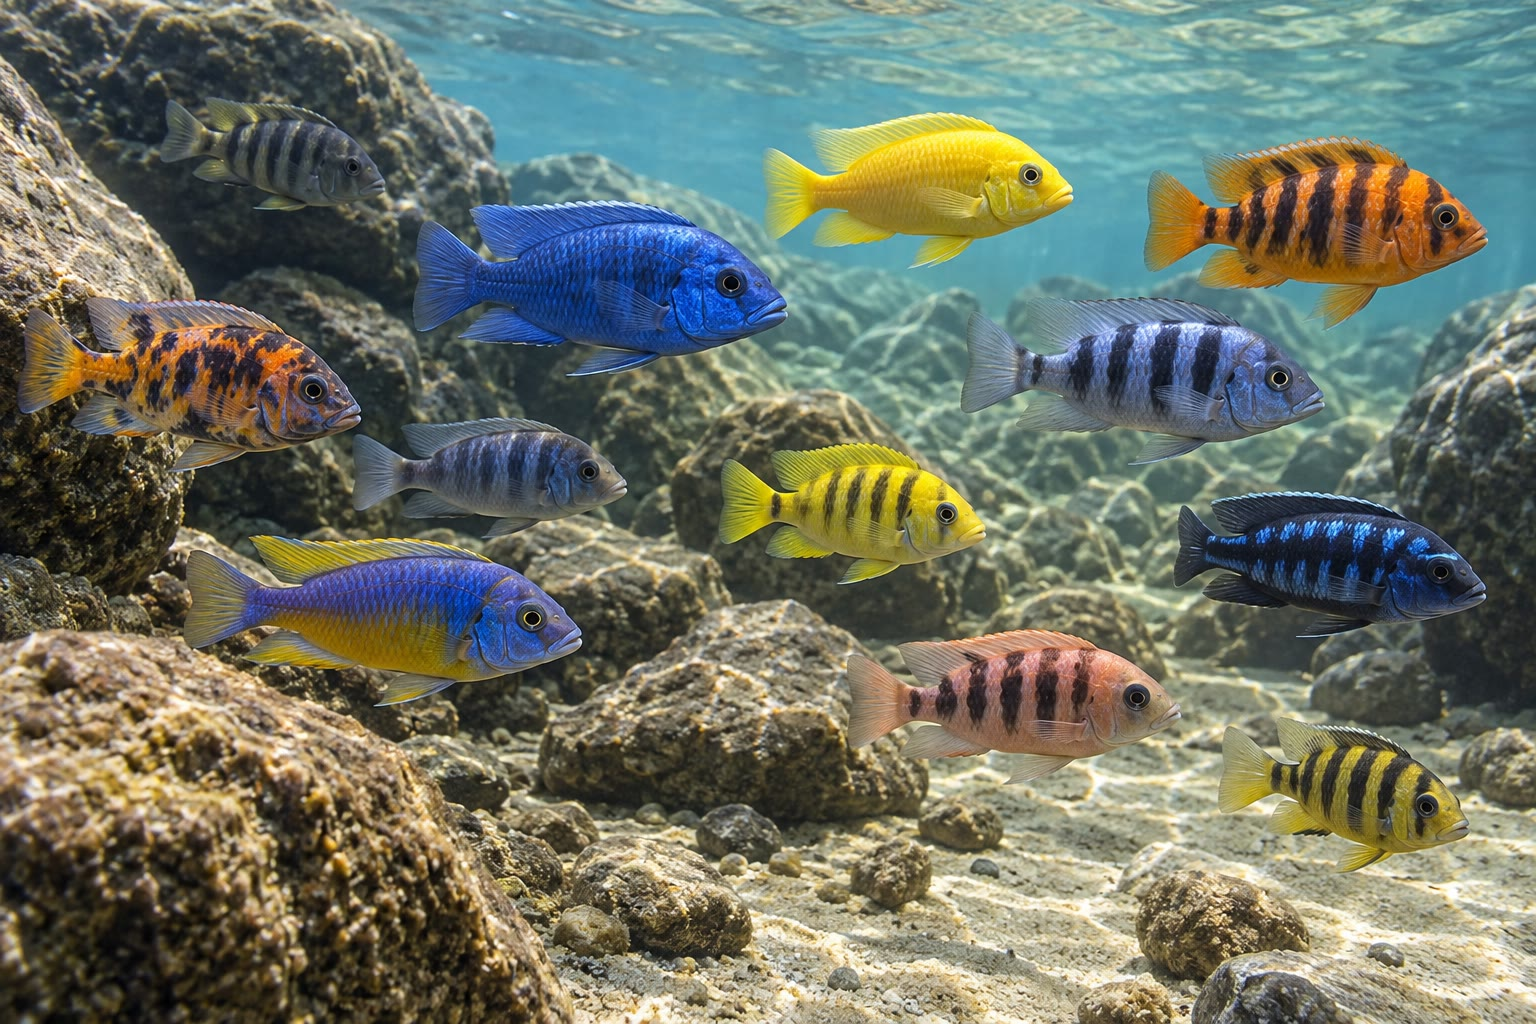
\includegraphics[width=0.6\linewidth]{images/book5/ai/b5-25-cichlids.jpg}

{\small Ikan siklid sebuah danau Afrika: ratusan spesies dalam beberapa
ribu tahun, dengan perbedaannya ditarik sebagian besar dari ragam yang sudah diusung
nenek moyang bersamanya.}
\end{omfigure}

\begin{remark}[Kebetulan sebagai dasarnya]\label{rem:b3:molecular-evolution:remark}
\omterm{thm:b3:molecular-evolution:neutral}{Teori netralnya} bukanlah sebuah klaim bahwa seleksi tidak penting; ia
sebuah pernyataan tentang apa yang terjadi ketika seleksinya tidak ada, yang cukup cermat
untuk diuji. Karena laju netralnya adalah laju mutasinya,
penyimpangannya mengukur waktu; karena perubahan netralnya mengisi tapak yang
dibiarkan bebas seleksinya, $\omega$ mengukur kekangannya; karena garis keturunan
netralnya berkoalesensi pada laju yang diketahui, ketaksesuaian \omterm{prop:b3:molecular-evolution:ils}{pohon gennya}
mengukur ukuran populasi yang tidak dilihat siapa pun. Seleksi lalu menjadi apa yang
tersisa ketika kebetulannya telah dikurangkan --- sebuah gen dengan $\omega$ di atas
satu, sebuah sapuan yang telah mengosongkan ragam dari sebuah daerah, sebuah pohon yang
tidak sesuai pada sebuah arah yang tidak dapat dijelaskan hanyutannya. Antibeku ikan es
Antarktika, lisozim lambung hewan pemamah biak, serta opsin ketiga primata
adalah kekecualian yang ditemukan dengan cara ini, dan masing-masing sebuah kisah sebuah gen
yang disalin dan sebuah tugas baru. Sisa genomnya adalah sebuah jam.
\end{remark}

\section{Latihan}

\begin{exercise}[$\star$]\label{exo:b3:molecular-evolution:1}
Nyatakanlah \omterm{thm:b3:molecular-evolution:neutral}{laju substitusi} netralnya lalu jelaskanlah dengan kata-kata mengapa ia tidak
bergantung pada ukuran populasinya.
\end{exercise}

\begin{exercise}[$\star$]\label{exo:b3:molecular-evolution:2}
Definisikanlah \omterm{def:b3:genomics:comparative}{ortolog}, \omterm{def:b3:genomics:comparative}{paralog}, dan \omterm{def:b3:molecular-evolution:duplication}{pseudogen}, dengan satu contoh masing-masing dari
keluarga globinnya.
\end{exercise}

\begin{exercise}[$\star$]\label{exo:b3:molecular-evolution:3}
Apa yang diukur $\omega = d_{N}/d_{S}$? Tafsirkanlah $\omega = 0.02$,
$\omega = 1.0$, dan $\omega = 2.5$, lalu namailah sebuah gen dari tiap jenisnya.
\end{exercise}

\begin{exercise}[$\star$]\label{exo:b3:molecular-evolution:4}
Mengapa Kimura menyimpulkan bahwa kebanyakan substitusinya netral? Nyatakanlah kembali
hujahnya dengan angka pada pembukaan bab ini.
\end{exercise}

\begin{exercise}[$\star\star$]\label{exo:b3:molecular-evolution:5}
$N = 5000$. Hitunglah \omterm{thm:b3:molecular-evolution:neutral}{peluang pemancangan} sebuah mutasi baru dengan $s
= 0$, $s = 0.001$, $s = 0.01$, dan $s = -0.001$, memakai rumus Kimura,
lalu berilah ulasan tentang mana yang netral efektif.
\end{exercise}

\begin{exercise}[$\star\star$]\label{exo:b3:molecular-evolution:6}
Dua spesies berbeda pada \qty{12}{\%} tapak sebuah gen yang laju
netralnya \qty{2e-9}{} tiap tapak tiap tahun. Taksirlah waktu penyimpangannya
dengan dan tanpa koreksi Jukes--Cantor. Pada selisih mentah berapa
koreksinya mencapai sebuah faktor dua?
\end{exercise}

\begin{exercise}[$\star\star$]\label{exo:b3:molecular-evolution:7}
Sebuah gen berkodon 300 punya 700 tapak nonsinonim dan 200 tapak sinonim.
Antara dua spesies ia menunjukkan 7 selisih nonsinonim dan 10 selisih sinonim.
Hitunglah $p_{N}$, $p_{S}$, dan $\omega$ (tanpa koreksi). Rezim
seleksi yang mana? Bagaimana bila cacahnya 35 dan 10?
\end{exercise}

\begin{exercise}[$\star\star$]\label{exo:b3:molecular-evolution:8}
Urutan netral manusia dan simpanse berbeda pada \qty{1.2}{\%}; perpisahannya
\qty{6.5}{Myr} lalu, dengan waktu angkatan \qty{25}{yr}. Taksirlah
laju mutasinya tiap tapak tiap angkatan, dan cacah mutasi baru
di dalam sebuah genom diploid berbasa $6\times 10^{9}$ tiap angkatan.
\end{exercise}

\begin{exercise}[$\star\star$]\label{exo:b3:molecular-evolution:9}
Dengan $N = \num{50000}$ dan $T = \num{100000}$ angkatan antara kedua
perpisahannya, hitunglah pecahan \omterm{prop:b3:molecular-evolution:ils}{pohon gen} yang tidak sesuai dengan
\omterm{prop:b3:molecular-evolution:ils}{pohon spesiesnya} bagi manusia, simpanse, dan gorila. $T$ berapa yang akan membuatnya
\qty{10}{\%}?
\end{exercise}

\begin{exercise}[$\star\star\star$]\label{exo:b3:molecular-evolution:10}
Tunjukkanlah bahwa rumus Kimura menyusut menjadi $1/2N$ ketika $s \to 0$ dan menjadi $2s$
bagi $4Ns \gg 1$, serta bahwa bagi $s < 0$ dengan $4N|s| \gg 1$ ia berlaku sebagai
$2|s|\,\mathrm{e}^{-4N|s|}$. Dari situ taksirlah seberapa kuat merugikan sebuah
mutasi harus, di dalam sebuah populasi $10^{4}$, agar \omterm{thm:b3:molecular-evolution:neutral}{peluang pemancangannya}
terpangkas seratus kali lipat di bawah netralnya.
\end{exercise}

\begin{exercise}[$\star\star\star$]\label{exo:b3:molecular-evolution:11}
Sebuah uji laju nisbi: sebuah kelompok luar $O$ berjarak terkoreksi $0.30$
dari mencit dan $0.24$ dari manusia, dan mencit serta manusia berjarak $0.20$. Hitunglah panjang
cabang mencit dan manusianya sejak perpisahannya (anggaplah titik perpisahannya berjarak sama dari
$O$ pada kedua jalannya), dan nisbahnya. Dengan sebuah angkatan mencit
\qty{0.5}{yr} dan angkatan manusia \qty{25}{yr}, apa yang akan diramalkan sebuah jam
tiap angkatan yang ketat bagi nisbahnya, dan apa yang dikatakan
pengamatannya tentang laju mutasi tiap angkatannya?
\end{exercise}

\begin{exercise}[$\star\star\star$]\label{exo:b3:molecular-evolution:12}
Sebuah gen yang tergandakan dilepaskan dari kekangannya ($\omega = 1$) pada
laju netral $k = \qty{2e-9}{}$ tiap tapak tiap tahun. Pada sebuah urutan penyandi
berbasa 1000, kira-kira berapa tahun sampai kodon henti atau
geseran kerangka yang pertama diharapkan (anggaplah sekitar \qty{4}{\%} mutasi titik acak
di dalam sebuah urutan penyandi menciptakan sebuah kodon henti, dan abaikanlah indel)?
Bandingkanlah dengan waktu yang dipunyai seleksi untuk menemukan sebuah fungsi baru, lalu jelaskanlah
mengapa kebanyakan gandaannya mati.
\end{exercise}

\section{Soal: Laju Perubahan}

\begin{problem}[{Soal akhir pekan --- sejarah sebuah genom dalam angka:
laju mutasi dari penyimpangan manusia--simpanse, beban
substitusi Kimura, peluang pemancangan mutasi yang terpilih, $\omega$ sebuah gen
dari cacah kodonnya, jam yang dibaca bagi sebuah penggandaan, serta
ketaksesuaian pohon gen di antara kera besar, berakhir pada laju mutasinya,
$\omega$ gennya, dan pecahan yang tak sesuainya}]
\label{pb:b3:molecular-evolution:1}
Data: penyimpangan netral manusia--simpanse $d = 0.012$; perpisahannya
\qty{6.5}{Myr} lalu; angkatan \qty{25}{yr}; genom diploid $6\times
10^{9}$ basa, \qty{1.5}{\%} penyandi. Populasi leluhurnya $N =
\num{50000}$. Gennya: 400 kodon, 920 tapak nonsinonim dan 280 tapak sinonim;
selisih manusia--mencitnya 46 nonsinonim dan 84 sinonim.
Perpisahan manusia--mencit \qty{90}{Myr}. Globin: $\alpha$ dan $\beta$ berbeda pada
\qty{55}{\%} tapak asam aminonya (mentah); laju hemoglobinnya \num{1e-9} tiap
tapak tiap tahun. Kera: $T$ antara perpisahan gorila dan simpansenya
\num{80000} angkatan. Batas Haldane: satu substitusi terpilih tiap
300 angkatan.

\medskip
\noindent\textbf{Bagian I --- Lajunya.}
\begin{enumerate}
  \item Dari $d = 2kT$, hitunglah $k$ tiap tapak tiap tahun, lalu $\mu$ tiap
        tapak tiap angkatan.
  \item Berapa mutasi baru tiap genom diploid tiap angkatan, dan berapa banyak di
        antaranya yang jatuh di dalam urutan penyandinya?
  \item Berapa substitusi yang terpancang tiap angkatan di seluruh genomnya pada
        laju netralnya (populasinya memancangkan $\mu$ tiap tapak tiap
        angkatan)? Bandingkanlah dengan batas Haldane lalu tariklah
        kesimpulan Kimura.
  \item Di dalam sebuah populasi $N = \num{50000}$, berapa mutasi netral baru
        yang timbul tiap tapak tiap angkatan di seluruh populasinya,
        dan berapa pecahannya yang akan pernah terpancang?
  \item Berapa lama sebuah mutasi netral yang ditakdirkan terpancang memakan waktu, dalam
        angkatan dan tahun? Bandingkanlah dengan waktu sejak
        perpisahan manusia--simpansenya.
  \item Jelaskanlah mengapa, meskipun ada pertanyaan~5, penyimpangan antara dua
        spesies mengukur waktu sejak perpisahannya dan bukan waktu
        sejak alelnya terpancang.
\end{enumerate}

\medskip
\noindent\textbf{Bagian II --- Peluang seleksinya.}
\begin{enumerate}[resume]
  \item Berapa \omterm{thm:b3:molecular-evolution:neutral}{peluang pemancangan} sebuah mutasi netral pada $N = \num{50000}$,
        dan sebuah mutasi dengan $s = 0.001$, $s = 0.01$, $s = 0.1$?
  \item Bagi $s$ yang mana $4Ns = 1$? Tafsirkanlah batasnya.
  \item Sebuah mutasi merugikan dengan $s = -0.001$: berapa \omterm{thm:b3:molecular-evolution:neutral}{peluang pemancangannya}
        relatif terhadap netralnya? Dan $s = -10^{-5}$?
  \item Bila sebuah pecahan $10^{-5}$ mutasi baru di dalam sebuah gen
        menguntungkan dengan $s = 0.01$ dan sisanya netral, berapa pecahan
        substitusi di dalam gen itu yang bersifat adaptif? Berilah ulasan tentang seberapa
        jarang seleksinya tampak pada urutannya bahkan ketika ia bekerja.
  \item Hitunglah $p_{N}$ dan $p_{S}$ bagi gen manusia--mencitnya, koreksilah
        masing-masing dengan Jukes--Cantor, lalu berikanlah $\omega$.
  \item Tafsirkanlah $\omega$; lalu taksirlah laju netral yang disiratkan
        $d_{S}$ gennya (tiap tapak tiap tahun) memakai waktu perpisahannya. Sesuaikah
        ia dengan pertanyaan~1?
\end{enumerate}

\medskip
\noindent\textbf{Bagian III --- Jam dan salinan.}
\begin{enumerate}[resume]
  \item Koreksilah selisih globin $\alpha$--$\beta$-nya bagi kenaan
        berganda (pakailah $d = -\ln(1 - p)$, yakni versi protein dengan banyak
        keadaan), lalu tanggalilah penggandaannya dengan laju hemoglobinnya.
  \item Tanggalnya jatuh dekat asal usul vertebrata berahang
        (\qtyrange{450}{500}{Myr}). Apa yang dimungkinkan punya rantai $\alpha$
        dan $\beta$ yang terpisah yang tidak dimungkinkan sebuah rantai tunggal?
  \item Fibrinopeptida berubah pada $8\times 10^{-9}$ tiap tapak tiap tahun.
        Dua spesies berpisah \qty{40}{Myr} lalu: berapa selisih mentah yang diharapkan?
        Mengapa protein ini tak berguna untuk menanggali perpisahan
        \qty{500}{Myr}?
  \item \omterm{def:b3:chromatin-epigenetics:nucleosome}{Histon} H4 berubah pada $10^{-11}$: berapa substitusi pada 100
        tapak sepanjang \qty{1000}{Myr}? Mengapa ia tak berguna untuk menanggali perpisahan
        yang baru?
  \item Sebuah gen gandaan hanyut dengan $\omega = 1$ sejak saat
        penggandaannya. Bila \qty{4}{\%} substitusi di dalam urutan penyandinya
        menciptakan kodon henti, dan gennya punya 1200 tapak pada laju $2\times
        10^{-9}$ tiap tapak tiap tahun, taksirlah harapan waktu sampai
        kodon henti yang pertama.
  \item Mengapa penggandaan genom utuh memberi gandaannya peluang
        bertahan hidup yang lebih baik daripada sebuah penggandaan tandem tunggal?
\end{enumerate}

\medskip
\noindent\textbf{Bagian IV --- Pohon di dalam pohon.}
\begin{enumerate}[resume]
  \item Berapa peluang sebuah garis keturunan manusia dan simpanse gagal
        berkoalesensi dalam \num{80000} angkatan sebelum perpisahan gorilanya?
  \item Berapa pecahan \omterm{prop:b3:molecular-evolution:ils}{pohon gen} yang tidak sesuai dengan \omterm{prop:b3:molecular-evolution:ils}{pohon spesiesnya}?
        Yang teramati: sekitar \qty{30}{\%}. Sesuaikah?
  \item Dari pohon yang tak sesuainya, berapa pecahan yang mengelompokkan manusia dengan
        gorila, dan berapa pecahan yang mengelompokkan simpanse dengan gorila? Apa yang akan ditunjukkan sebuah
        penyimpangan yang kuat dari kesamaannya?
  \item Bila populasi leluhurnya $N = \num{10000}$, pecahan yang tak
        sesuai berapa yang akan Anda harapkan? Apa yang karena itu dikatakan pecahan yang teramati
        tentang cacah nenek moyang kita?
  \item Mengapa merangkai seribu gen menjadi satu \omterm{def:b3:bioinformatics:alignment}{penjajaran} memberi
        sebuah pohon yang meyakinkan tetapi mungkin salah, dan apa yang justru dilakukan sebuah
        metode koalesen?
  \item DNA Neanderthal pada manusia non-Afrika sekitar \qty{2}{\%} dan
        pohon yang mengusungnya mengelompokkan sebagian orang Eropa dengan Neanderthal lebih
        sering daripada orang Afrika. Mengapa ini bukan pemilahan garis keturunan yang tak lengkap?
  \item Ringkaslah: $\mu$ (pertanyaan~1), $\omega$ gennya
        (pertanyaan~11), dan pecahan yang tak sesuainya (pertanyaan~20).
\end{enumerate}
\end{problem}
